\section{Smooth Surfaces}
\label{sec:smooth-surfaces}

In this section, we discuss the sphere and the plane, we highlight differences and similarities,
 and discuss maps between surfaces.

\subsection{The plane and the sphere}

Before discussing the plane and the sphere let us first strengthen our intuition in 
one dimension with the real number line and the unit circle.
Often, we think of the real line $\R$ and the unit circle $\Sp^1$ as subsets of $\R^2$,
the line is the set
$$\R^1=\{(x,y)\in \R^2 | y=0\}$$
and the unit circle is the set
$$\Sp^2=\{(x,y)\in \R^2 | x^2+y^2=1\}.$$
In formally, the line and the circle are one dimensional because
we only need one coordinate to specify any point on them.
Is it possible to continuously deform the circle into the line?
The answer is no, as we will see.
There is a map, stereographic projection, between all but one point on the circle
and the line.


Consider a line from the north pole of the unit circle $(0,1)$ that intersects
the unit circle at the point $(u,v)$ parameterized by $p(t)=(1-t)(0,1)+t(u,v).$
By considering the $y$-coordinate we determine the $t$ value were $p(t)$
intersects the $x$-axis, namely $t=\frac{1}{1-v}.$ Then, 
the $x$-coordinate where $p(t)$ intersects the real line is 
$$x=\frac{u}{1-v}.$$ An example is shown
in \figref{stereo1D}.

\begin{figure}[htb]
	\centering
	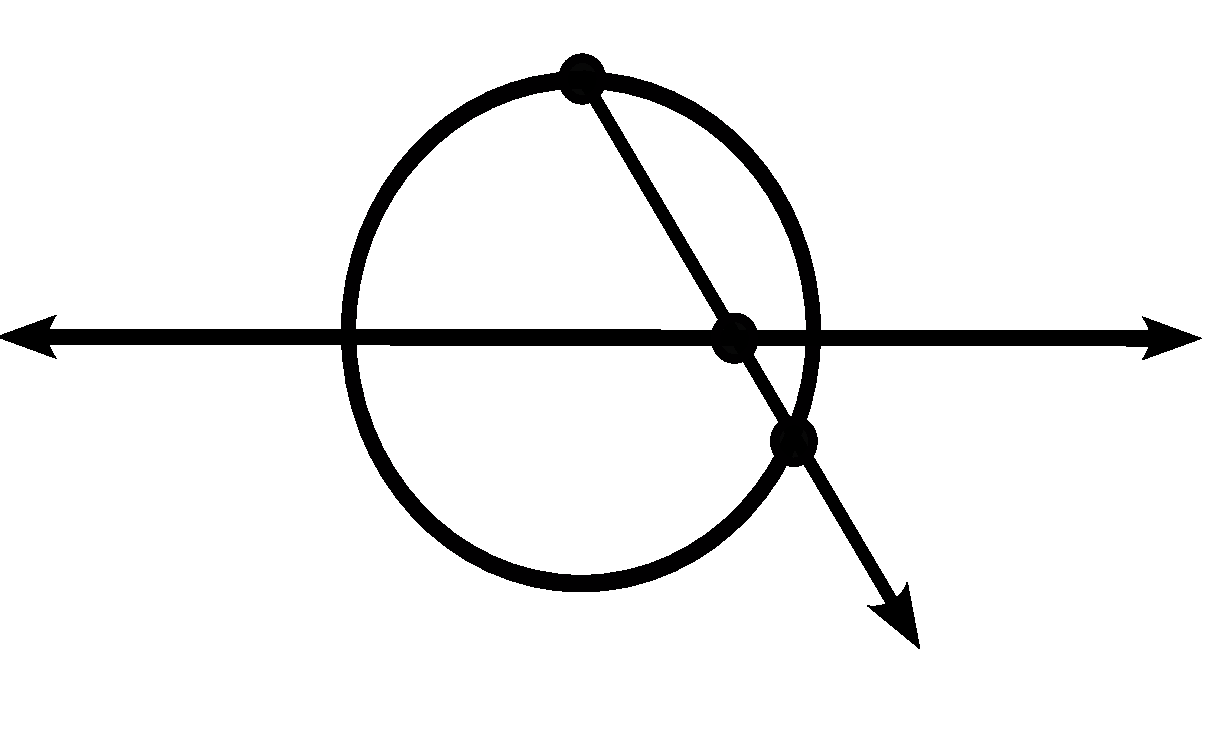
\includegraphics[width=.3\textwidth]{curvature/stereo-1D}
	\caption{One dimensional stereographic projection.}
	\label{fig:stereo1D}
\end{figure}

A similar argument can be used to find the inverse map from
the real line to the unit circle. Given an $x$-value on the real line we consider
the parameterized line $p^{-1}(t)=(1-t)(0,1)+t(x,0)$ and compute
the $t$ value where $p^{-1}$ is on the unit circle and $t\neq 0.$ We find
$t=\frac{2}{1+x^2}$ and the point $(u,v)$ on the unit circle in terms of $x$ is
$$u=\frac{2x}{1+x^2}, v=\frac{x^2-1}{1+x^2}.$$

We now consider the same idea in dimension two.
We often think of the sphere and the plane as subsets of $\R^3$,
the sphere is the set
$$\Sp^2=\{(x,y,z)\in \R^3 | x^2+y^2+z^2=1\}$$
and the $xy$-plane is
$$\R^2=\{(x,y,z)\in \R^3 | z=0\}.$$
Is it possible to continuously deform the sphere into the plane?
Again, the answer is no, but we define stereographic projection between all but one point
 on the sphere and the plane analogously to the one dimensional case.
 Given a point $p$ on the sphere, we draw a straight line
from the north pole $N=(0,0,1)$ through $p$, then find the intersection of
this line with the plane. Every point on the sphere is mapped
to a unique point in the plane except of the north pole.
See \figref{stereo1} for an illustration.





\begin{figure}[htb]
	\centering
	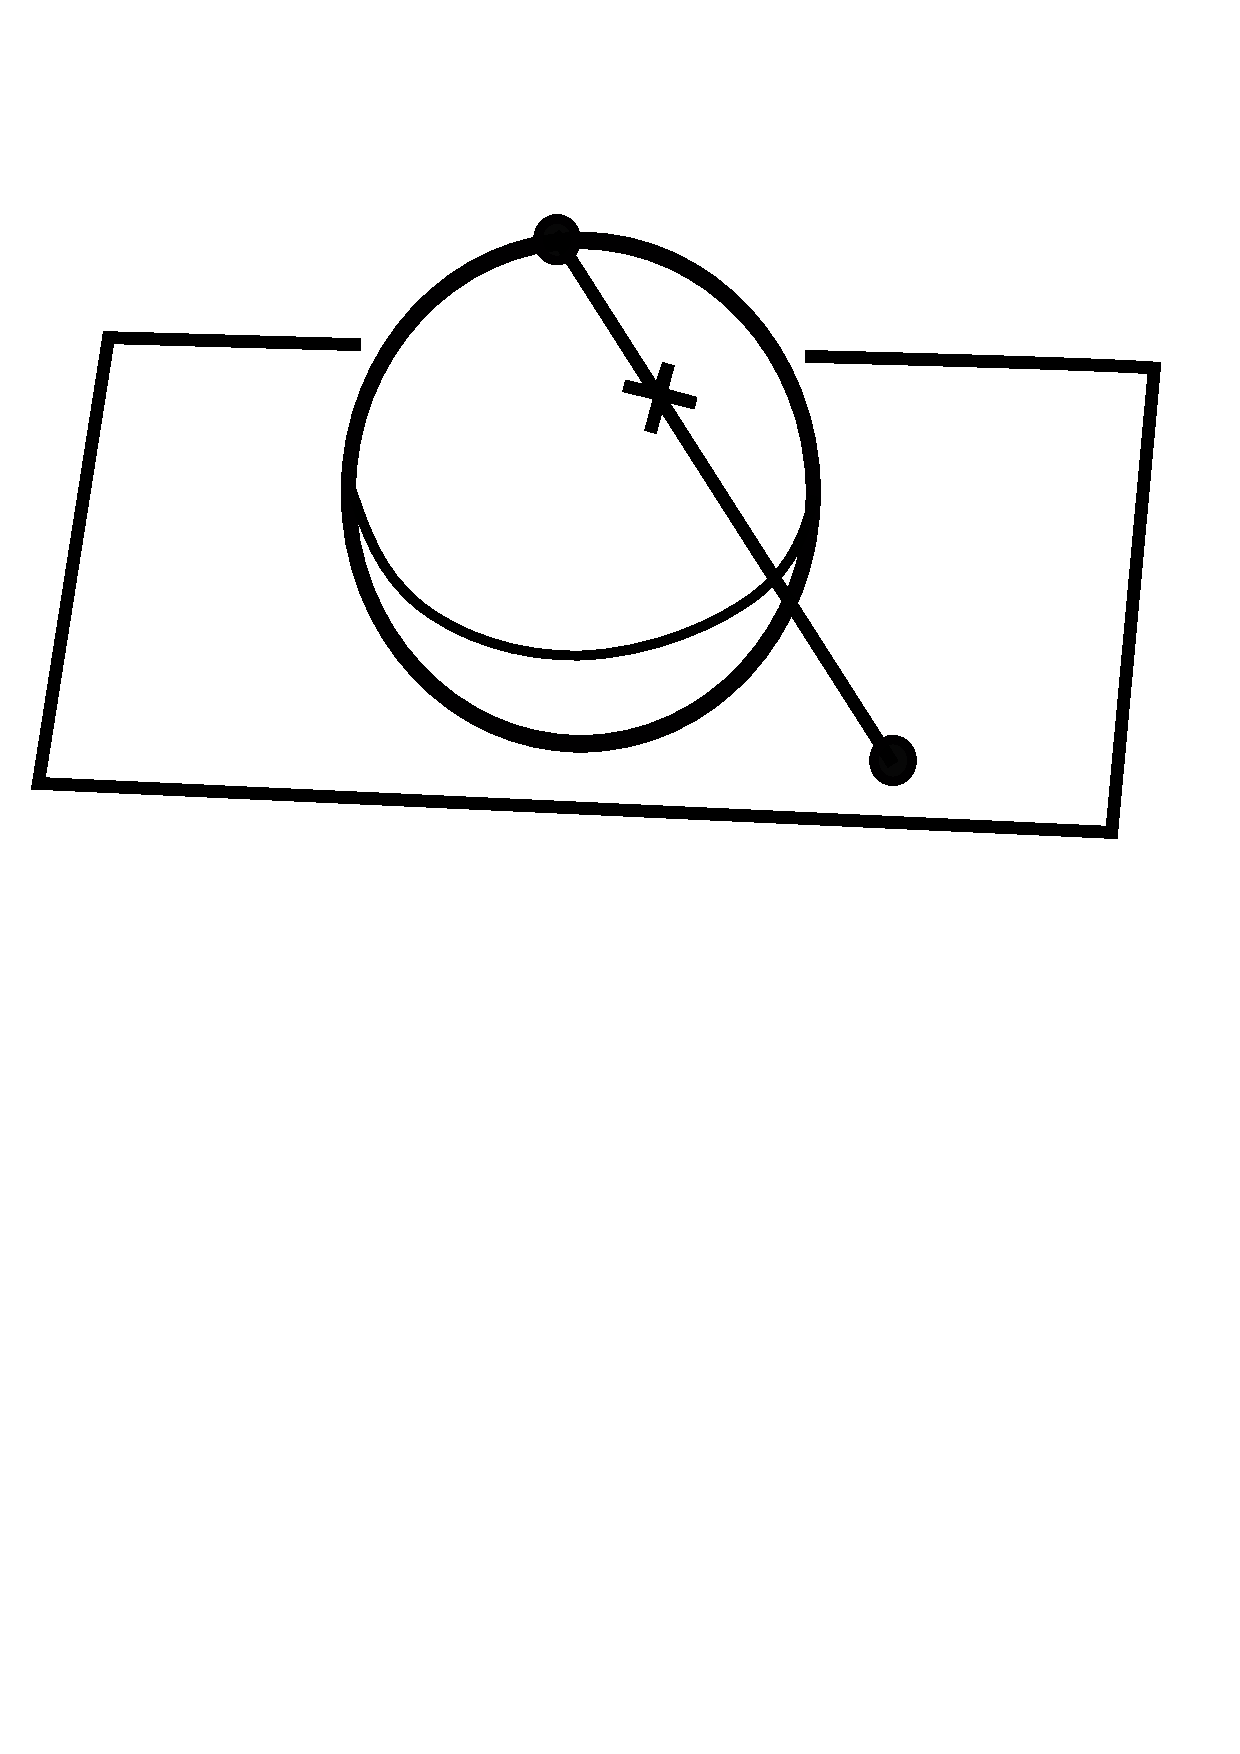
\includegraphics[width=.3\textwidth]{curvature/stereo}
	\caption{A point on the sphere is mapped to a point on the plane by stereographic projection.}
	\label{fig:stereo1}
\end{figure}


We are able to obtain formulas for stereographic projection from
the unit sphere to the plane as follows \cite{christian-notes}.
The line from the north pole $(0,0,1)$ that intersects $(x,y,z)\in \Sp^2$ parametrized by 
$p(t)=(1-t)(0,0,1)+t(x,y,z)$. By considering the $z$ coordinate we determine the $t$ value where this line
intersects $\R^2$, namely $t=\frac{1}{1-z}.$
This gives the desired map  and in equation form we have
$$p(x,y,z)\to \left(\frac{x}{1-z},\frac{y}{1-z}\right).$$



Many of us have more experience doing computations on $\R$ and $\R^2$ as opposed
to other objects. Stereographic projection enables us to transform problems on
the circle and the sphere into problems in $\R$ and $\R^2$ respectively.

\subsection{Stereographic Projection is Conformal}


Stereographic projection has the property that it preserves angles.
Maps with this property are called conformal. 
\begin{definition}[Conformal]\label{def:conformal}
	Let $U$ and $V$ be open subsets of $\R^n$, a function $f:U\to V$ is
	\emph{conformal} at a point $u\in U$ if it preserves angles between curves
	through $u$ and preserves orientation.
\end{definition}

Now we prove that stereographic projection is conformal following \cite{hilbert-imagination}.
Our secondary goal is to review ideas from calculus that will be useful later.

What does it mean for a function to be differentiable? Let $g:\R\rightarrow \R$ be single variable function that is differentiable at a point $q$. Informally, being differentiable at a point means that the tangent
line through that point gives a `good' approximation of $f$ for points near $q$. We can use a linear map to approximate $f$. 

Now, consider two smooth surfaces $S_1$ and $S_2$ with $f:S_1\rightarrow S_2.$ Since our
surfaces are smooth, we can locally approximate them with a tangent planes. 
For $p\in S_1$, we denote the tangent plane at $p$ by $T_pS_1.$ If we want a vector in $T_pS_1$,
we can consider a smooth curve $\gamma(t)\in S_1$ with $\gamma(t_0)=p$, then $\gamma'(t_0)$ 
is in $T_pS_1.$ Choosing another curve though $p$ with derivative linearly independent of $\gamma'(t_0)$
gives a basis for $T_pS_1$.
Since $\gamma(t)$ is a smooth curve on $S_1$, then $f\circ \gamma(t)$ is a smooth curve
on $S_2$ that passes through $f(p)\in S_2.$
We can approximate $f$ near $p$ with a linear map form $df_p:T_pS_1\rightarrow T_{f(p)}S_2.$
The map $df_p$ tells us how vectors at $p$ are mapped to vectors at $f(p).$

A property we will use in our proof is that tangent vectors of $\gamma(t_0)$ are mapped
to tangent vectors at $f(p)$. To see this, suppose $\gamma'(t_0)\in T_pS_1$ and
$(f\circ \gamma)'(t_0)\in T_{f(p)}S_2$ is a tangent vector at $f(p)$. But
$(f\circ \gamma)'(t_0)=df_p(\gamma'(t_0)),$ thus the differential $df_p$ maps
tangent vectors at $p$ to tangent vectors at $f(p).$




\begin{theorem}[Stereographic projection is conformal]\label{thm:stereo-confroms}
Stereographic projection is conformal.
\end{theorem}
\begin{proof}
	Let $p\in\Sp^2$ that is not the north pole, and let $T_p$ denote the tangent
	plane at $p$ and let $\pi$ denote stereographic projection.
	 We assume that $p$ is in the $xz$-plane, we rotate the sphere if it is not.
	The triangle formed by the origin, the north pole and $p$
	is an isosceles triangle. 
	The line from the origin through $p$ is normal to the sphere and perpendicular
	to $T_p$. Thus, the triangle formed by the line through $p$ and the north pole,
	$T_p$ and the $xy$-plane is an isosceles triangle, call this length $\ell$, 
	see \figref{conforms} for an illustration.
	
	Let $\gamma$ be any smooth curve through $p$, and let $\vec{t}$ be the tangent vector at $p$, then,
	 provided $\vec{t}$ isn't parallel to the $xy$-plane, one of $\pm \vec{t}$
	intersects the $xy$-plane. Let $\vec{t'}$ denote the intersection of the plane containing the north
	pole and $\vec{t}$ with the $xy$-plane. Since $\pi$ is differentiable, $\vec{t'}$ is tangent to $\pi \circ \gamma$ at $\pi(p)$. 
	Now $\gamma$ and $\vec{t}$ are curves in $\R^3$, and they have the same tangent, $\vec{t}$
	at $p,$ so $\pi\circ \gamma$ and $\pi \circ \vec{t}$ are curves in the $xy$-plane with the same
	tangent at $\pi(p),$ namely $\vec{t'}.$
	
	Let $\theta$ denote the angle formed by $\vec{t}$ and the $xz$-plane. 
	By the discussion
	above, the angle between $\vec{t'}$ and $\pi \circ \gamma$ is also $\theta$ by similar right triangles,
	see \figref{project-tangent}.
	In order for $\pi$ to be conformal it must preserve angle between two curves, so we repeat 
	the same argument of a second path $\gamma'$.
	
	
\end{proof}

 \begin{figure}[htb]
         \centering
        \begin{subfigure}[b]{0.4\textwidth}
         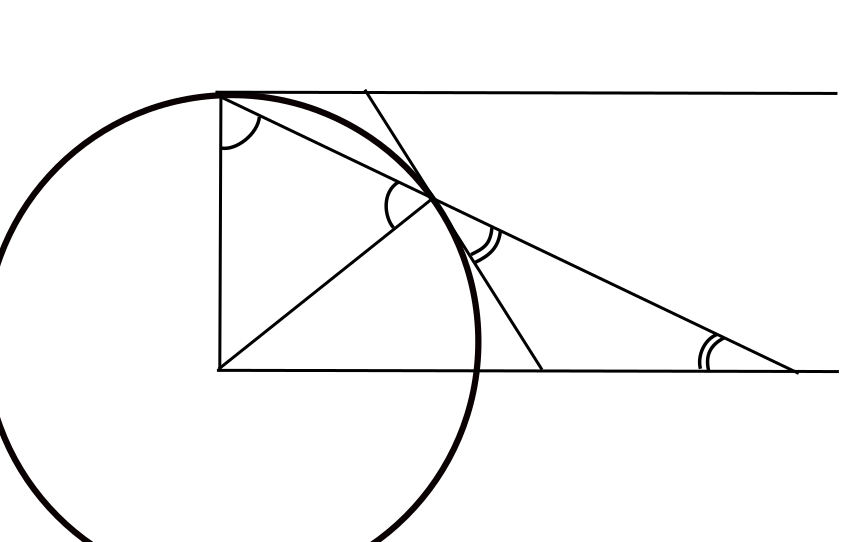
\includegraphics[width=\textwidth]{background/stero-conforms}
         \caption{}
 	 \label{fig:conforms}
       \end{subfigure}
         \hspace{1cm}
         \begin{subfigure}[b]{0.3\textwidth}
         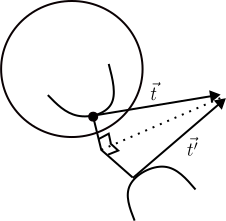
\includegraphics[width=\textwidth]{background/stero-conforms-2}
         \caption{}
          \label{fig:project-tangent}
         \end{subfigure}
		\caption{An illustration of the triangles discussed in proof of \thmref{stereo-confroms}
 		\label{fig:conformal}}
 \end{figure}


	
\subsection{Differences Between the Sphere and the Plane}

Now we highlight differences between the plane and the sphere.
In the plane, if one scales a polygon, the area of the polygon changes
but the angles of the polygon do not.
On the unit sphere, we can relate the area of a simple polygon 
to the angles. This is because the sphere is curved.
A triangle on the sphere is shown in \figref{sphere-triangle}.


 \begin{figure}[htb]
         \centering
        \begin{subfigure}[b]{0.35\textwidth}
         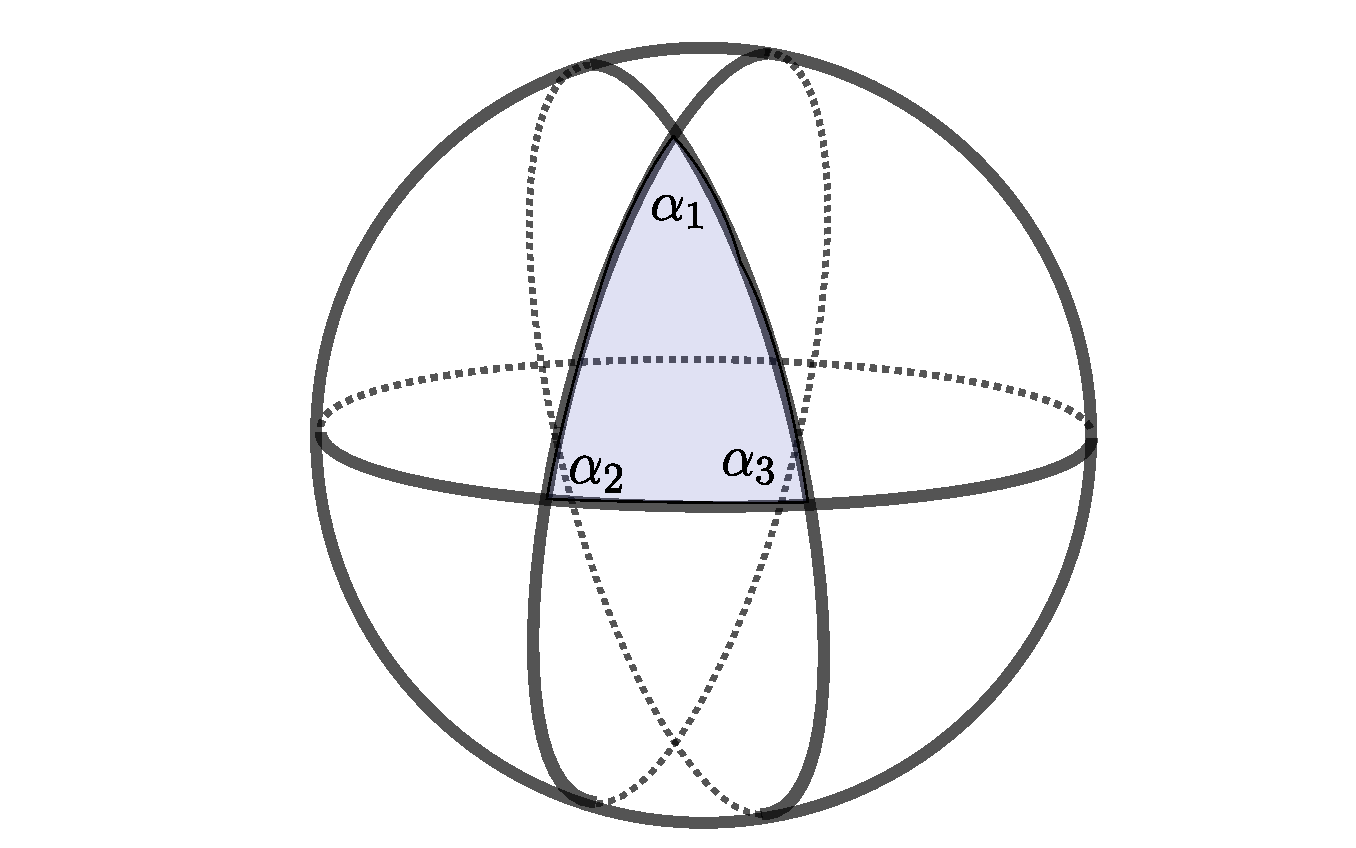
\includegraphics[width=\textwidth]{background/sphere-triangle}
         \caption{Spherical triangle.}
 	 \label{fig:sphere-triangle}
       \end{subfigure}
         \hspace{1cm}
         \begin{subfigure}[b]{0.35\textwidth}
         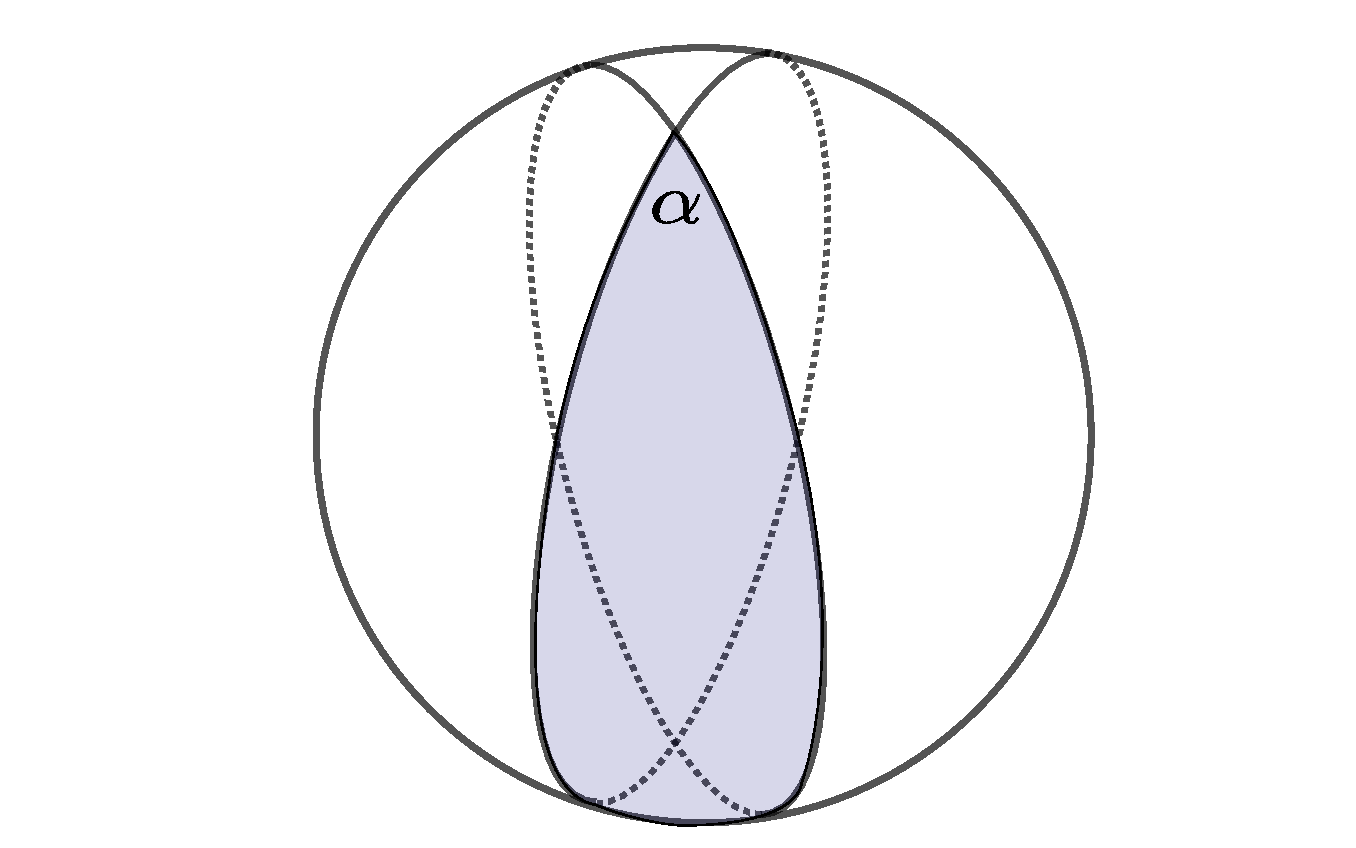
\includegraphics[width=\textwidth]{background/lune}
         \caption{A lune.}
          \label{fig:lune}
         \end{subfigure}
		\caption{(a) A triangle on the sphere.
 		(b) A lune with angle $\alpha$.
 		\label{fig:sphere-lune}}
 \end{figure}
A spherical \EMPH{lune} is the region on a sphere bounded by two half great circles
with angle $\alpha$. The area of a lune is denoted $A(\alpha)$,
 see \figref{lune}.
On the unit sphere, the area of a lune is proportional to $\alpha$. 
If $\alpha=0$ the area is zero and if $\alpha=\pi$ the area is $4\pi$.
We can add the area of two lunes in terms of their angles, 
$A(\alpha_1+\alpha_2)=A(\alpha_1)+A(\alpha_2)$ so $A$ is linear
and  $A(\alpha)=4\alpha.$




The following relates the area of a triangle on the sphere to the angles.

\begin{lemma}[Area of Spherical Triangle]\label{lem:spherical-triangle}
On the unit sphere, the area of a triangle with interior angles $\alpha_1, \alpha_2, \alpha_3$
is $A=\alpha_1+\alpha_2+\alpha_3-\pi$.
\end{lemma}

\begin{proof}
	Any two edges of the triangle form a lune. The collection of 
	all three lunes covers the entire sphere with triangle and the antipodal triangle covered three times.
 	The surface area of the unit sphere is $4\pi$.
	Thus, $4\pi=4\alpha_1+4\alpha_2+4\alpha_3-4A$
	and $A=\alpha_1+\alpha_2+\alpha_3-\pi$.
	
\end{proof}

As in the plane, any polygon on the sphere with $n$ vertices can be decomposed
into $n-2$ triangles \cite{orourke_computational_1994}. This gives a formula for the area of a simple polygon
on the sphere with interior angles $\alpha_1,\alpha_2,\ldots, \alpha_n$.

\begin{equation} \label{eqn:sphere-area}
	A=(2-n)\pi +\sum_{i=1}^n \alpha_i.
\end{equation}


Next, we explore how the area of disks changes as a function 
of the radius in the plane and on the sphere. 
In the plane, the area of a disk of radius $r$ is, of course,
$$A_{\R^2}(r)=\pi r^2.$$ However, this is not the case for the sphere where
the radius of the disk curves along the surface. Such a disk on the sphere
centered at a point $p$
is called a geodesic disk with intrinsic radius $r$.

Consider a sphere of radius $R$ and choose any point on the sphere $p.$
Recall, the length of an arc $\ell$ on a circle of radius $R$ with central angle $\theta$
is $\ell=\theta R.$ So, if we have a geodesic disk centered at $p$, with intrinsic radius $r$ with
$0<r<\pi R$,
the central angle between $p$ and a point on the boundary of the disk is 
$\theta=\frac{r}{R}.$ We can now integrate with spherical coordinates 
to determine the area of the geodesic disk to obtain

\begin{equation} \label{eqn:sphere-disk-area}
	A_{\Sp^2}(r)=\int_0^{2\pi}\int_0^{\frac{r}{R}}\sin(\phi)d\phi d\theta = 2\pi R^2\left(1-\cos\left(\frac{r}{R}\right)\right).
\end{equation}

If we consider the rate of change in the area of disks as a function of the radius
we see that, as the radius increases, the area increases slower on the sphere
than in the plane. 
In the plane $\frac{d}{dr}A_{\R^2}(r) =2\pi r$ and in the sphere
$$\frac{d}{dr}A_{\Sp^2}(r)=2\pi R\sin \left(\frac{r}{R}\right).$$
Since $0<r<\pi R$ and $0<\sin\left(\frac{r}{R}\right)< \frac{r}{R}$ we have

$$\frac{d}{dr}A_{\Sp^2}(r)=2\pi R\sin \left(\frac{r}{R}\right)<2\pi R \frac{r}{R}=\frac{d}{dr}A_{\R^2}(r).$$


\noindent \textbf{Exercises}


\begin{enumerate}
	\item Compute the derivative of stereographic production at the point $(\frac{\sqrt{2}}{2},0,\frac{\sqrt{2}}{2})$.
	
	\item Prove that stereographic projection maps circles to circles.
	
	\item Explain why integration using spherical coordinates includes the factor $\sin(\phi).$
	
\end{enumerate}

\pagebreak